\documentclass{article}

\usepackage{graphicx}
\usepackage{tikz}
\usepackage{tikzsymbols}
\usetikzlibrary{calc,patterns,shapes.geometric}
\pagestyle{empty}
\usepackage[margin=0pt]{geometry}
\geometry{papersize={14in,12in}}

\def\centerarc[#1](#2)(#3:#4:#5){\draw[#1] ($(#2)+({#5*cos(#3)},{#5*sin(#3)})$) arc (#3:#4:#5);}

\begin{document}
	\begin{figure}
		\centering
		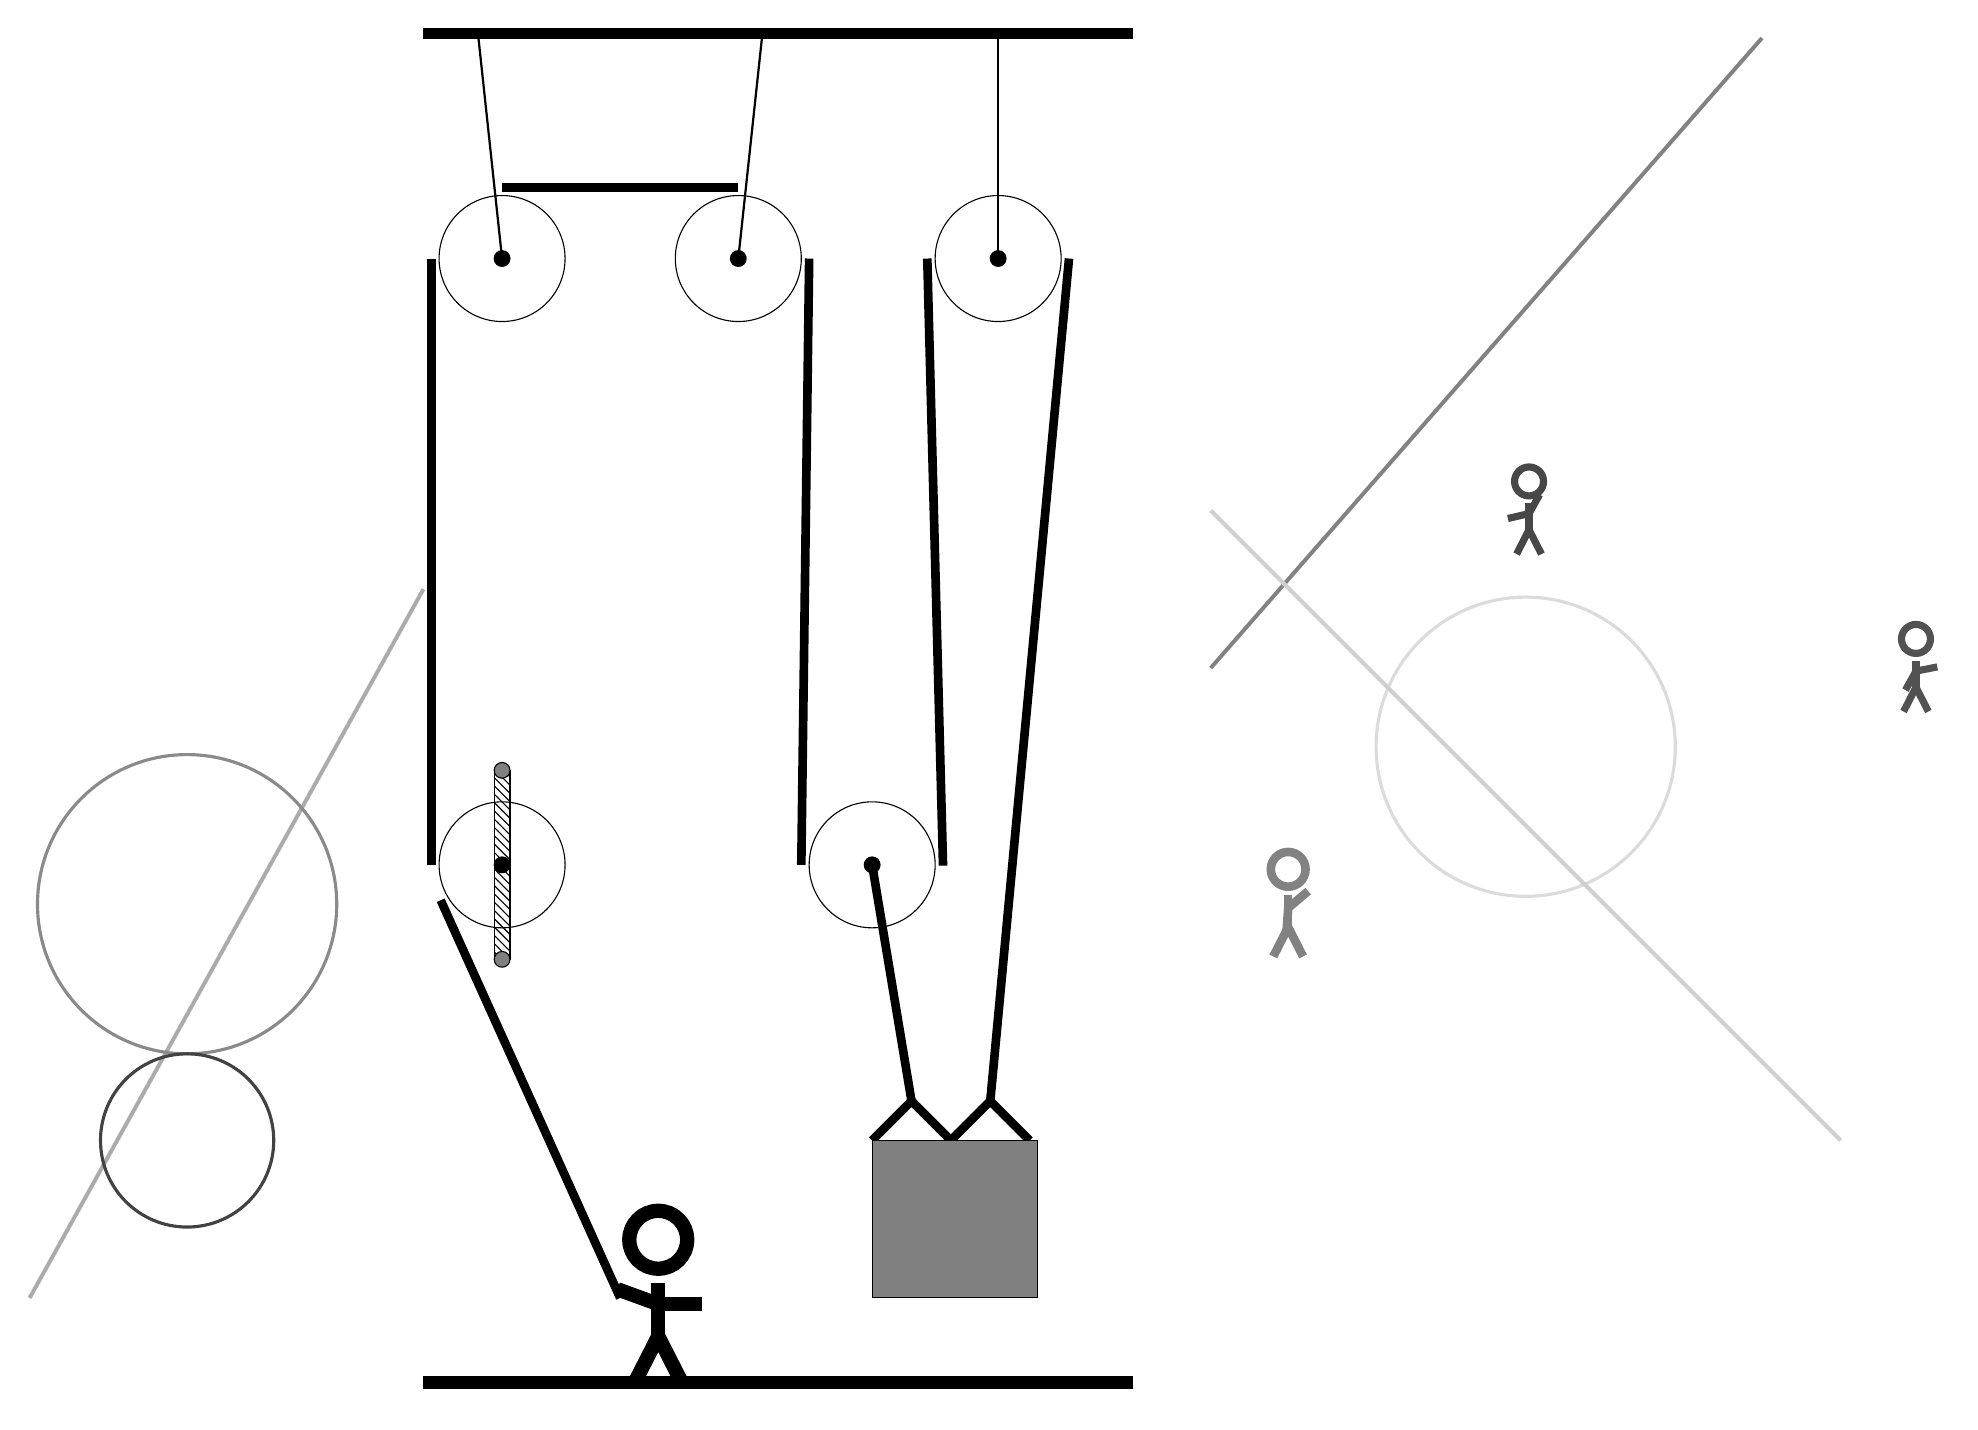
\begin{tikzpicture}
			%%%%% START %%%%%
			
			\draw[fill=black] (-3, 14) rectangle (6, 14.125);
			
			\draw (1, 11.2) circle (0.8);
			\draw[fill=black] (1, 11.2) circle (0.1);
			\draw[thick] (1, 11.2) -- (1.3, 14);
			
			\node[line width=0.3mm, color=black!49] at (8, 3) {\Strichmaxerl[6][86][40]};
			
			\node[line width=0.7mm, color=black!68] at (16, 6) {\Strichmaxerl[5][61][11]};
			\draw[line width=0.5mm, color=black!33](-3, 7) -- (-8, -2);
			\draw [line width=0.4mm, color=black!46](-6, 3) circle (1.9);
			
			\draw[line width=0.5mm, color=black!49](7, 6) -- (14, 14);
			\draw [line width=0.4mm, color=black!14](11, 5) circle (1.9);
			\node[line width=0.2mm, color=black!72] at (11, 8) {\Strichmaxerl[5][13][61]};
			
			\draw [line width=0.4mm, color=black!74](-6, 0) circle (1.1);
			\draw[line width=0.5mm, color=black!19](7, 8) -- (15, 0);
			
			\draw (4.3, 11.2) circle (0.8);
			\draw[fill=black] (4.3, 11.2) circle (0.1);
			\draw[thick] (4.3, 11.2) -- (4.3, 14);
			
			\draw (2.7, 3.5) circle (0.8);
			\draw[fill=black] (2.7, 3.5) circle (0.1);
			
			\draw[line width=1.1mm]  (2.7, 0) -- (3.2, 0.5) -- (3.7, 0) -- (4.2, 0.5) -- (4.7, 0);
			\draw[fill=black!50] (2.7, 0) rectangle (4.8, -2);
			
			\draw (-2, 11.2) circle (0.8);
			\draw[fill=black] (-2, 11.2) circle (0.1);
			\draw[thick] (-2, 11.2) -- (-2.3, 14);
			
			\draw (-2, 3.5) circle (0.8);
			\draw[fill=black] (-2, 3.5) circle (0.1);
			\draw[pattern=north west lines, pattern color=black] (-2.1, 4.7) rectangle (-1.9, 2.3);
			\draw[fill=black!50] (-2, 4.7) circle (0.1);
			\draw[fill=black!50] (-2, 2.3) circle (0.1);
			
			\draw[line width=1.1mm](-0.5, -2) -- (-2.7794, 3.05);
			\centerarc[line width=1.1mm](-2, 3.5)(180:210:0.9);
			\draw[line width=1.1mm](-2.9, 3.5) -- (-2.9, 11.2);
			\centerarc[line width=1.1mm](-2, 11.2)(90:180:0.9);
			
			\draw[line width=1.1mm](-2, 12.1) -- (1, 12.1);
			\centerarc[line width=1.1mm](1, 11.2)(0:90:0.9);
			\draw[line width=1.1mm](1.9, 11.2) -- (1.8, 3.5);
			\centerarc[line width=1.1mm](2.7, 3.5)(180:370:0.9);
			\draw[line width=1.1mm] (3.6, 3.49) -- (3.4, 11.2);
			\centerarc[line width=1.1mm](4.3, 11.2)(0:180:0.9);
			\draw[line width=1.1mm](4.2, 0.5) -- (5.2, 11.2);
			\draw[line width=1.1mm] (3.2, 0.5) -- (2.7, 3.5);
			
			\node at (0, -2) {\Strichmaxerl[10][-20][0]};
			
			\draw[fill=black] (-3, -3) rectangle (6, -3.15);
			
			%%%%% END %%%%%
		\end{tikzpicture}
	\end{figure}	
\end{document}